\section{Scale Factor Comparison Method}
\label{sec:comparison}

There are multiple montecarlo generators available for producing samples for use with ATLAS analyses. Since each generator has its own strengths and weaknesses the differences between them can be used to estimate the uncertainty associated with any mis-modelling produced by the generator.

As already mentioned the signal region in a higgs analysis is built from a series of cuts designed to reduce the contribution from processes such as Z$\rightarrow\tau\tau$ Typically this leads to large variations in the Z+jets differential distributions. The statistical variations can be controlled by including a Z enhanced control region into the likelihood fit. The data MC agreement can be then quantified by use of a normalisation factor. 

Figure [\ref{fig:lepPt0ZCR}] shows the distribution of Z$\rightarrow\ell\ell$ in an enhanced Z region. This is defined as being a window in the visible mass of 10GeV around the Z rest mass. Each cut gives slightly different agreement between data and mc section \ref{sec:zll} goes into more detail on this. Even in this `clean' Z region there is not a perfect agreement between data and MC. As such we can propagate this `known' difference between data and MC from the control region to the signal region through the use of a Normalisation Factor (NF though also known as a Scale Factor SF) this can be defined as:

\begin{equation}
\mathrm{PN^{SR}_{Z}=\frac{N^{SR}_{Z,MC}}{N^{SR}_{Z,MC}}\cdot(N^{CR}_{data}-N^{CR}_{nonZ})=TF_{Z}\cdot(N^{CR}_{data}-N^{CR}_{nonZ})}
\end{equation}

where $\mathrm{N^{CR}_{Z,MC},N^{CR}_{Z,MC}}$ etc are the expected number of Z/$\gamma$ events in signal and control regions. The difference in the transfer factor as calculated for difference generators can be taken as the generator modelling error. This can be calculated for any definition of the Z control region. Table \ref{table:uncertainties} shows the associated uncertainties taken from using Sherpa as the nominal generator for the Z$\rightarrow\ell\ell$ process. 


\begin{figure}[h!]
  \centering
   \subfloat[]{  
   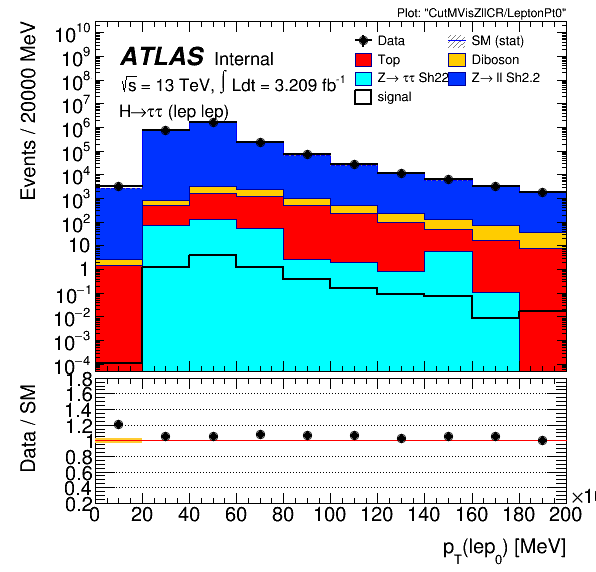
\includegraphics[width=0.4\textwidth]{figures/v05/sherpa22/eemm-CutMVisZllCR-LeptonPt0-log}
   }
   \subfloat[]{  
   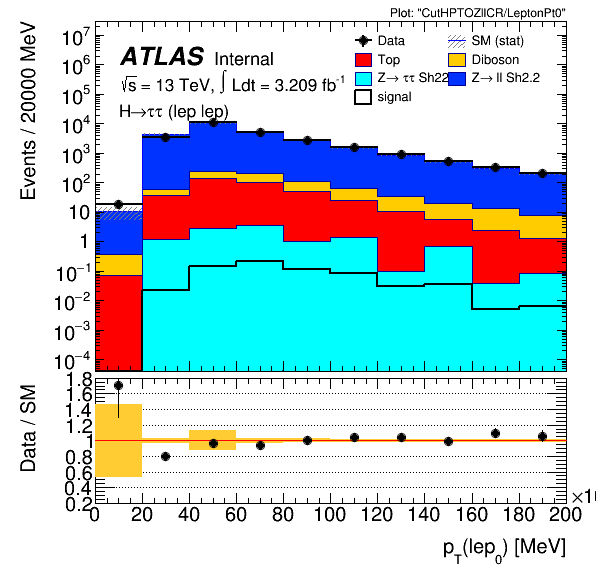
\includegraphics[width=0.4\textwidth]{figures/v05/sherpa22/eemm-CutHPTOZllCR-LeptonPt0-log}
   }\\
   \subfloat[]{  
   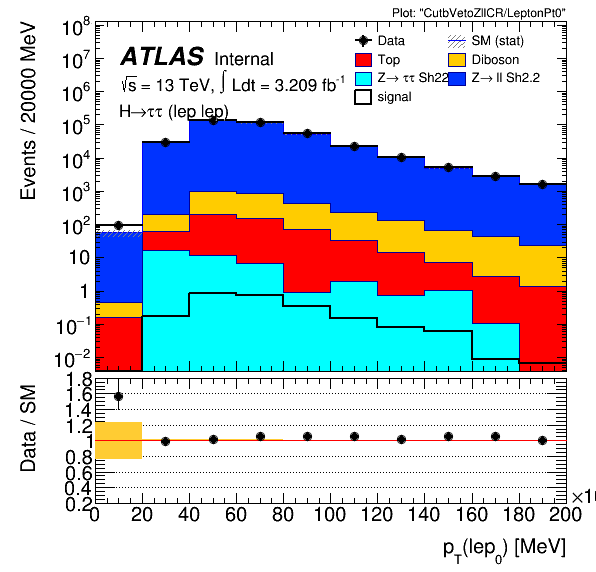
\includegraphics[width=0.4\textwidth]{figures/v05/sherpa22/eemm-CutbVetoZllCR-LeptonPt0-log}
   }
   \subfloat[]{  
   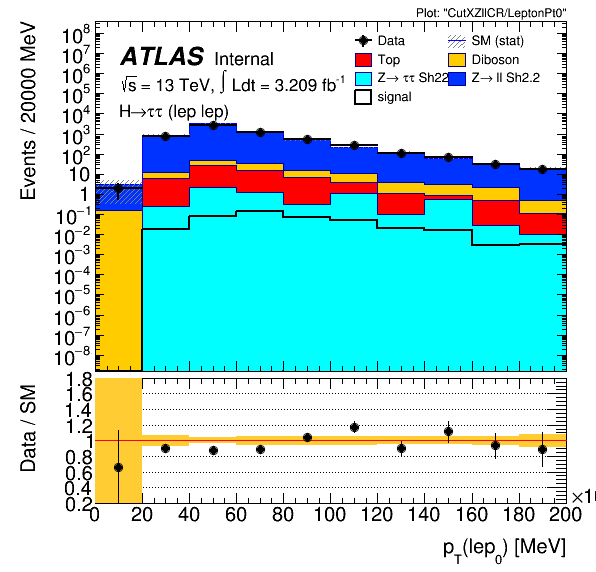
\includegraphics[width=0.4\textwidth]{figures/v05/sherpa22/eemm-CutXZllCR-LeptonPt0-log}
   }\\
   \subfloat[]{  
   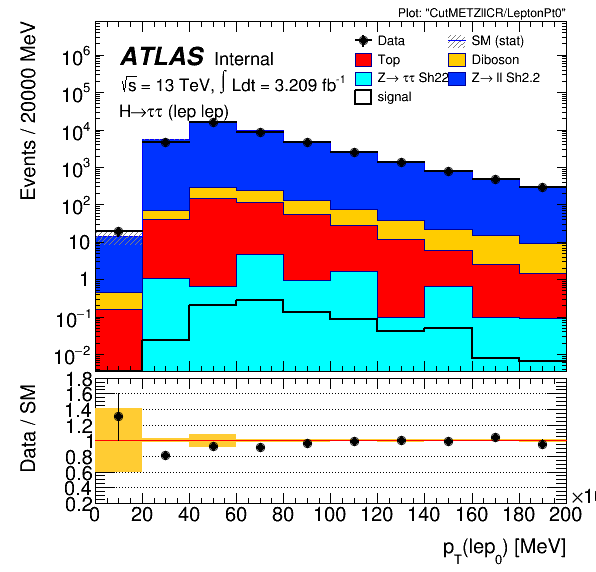
\includegraphics[width=0.4\textwidth]{figures/v05/sherpa22/eemm-CutMETZllCR-LeptonPt0-log}
   }
   \subfloat[]{  
   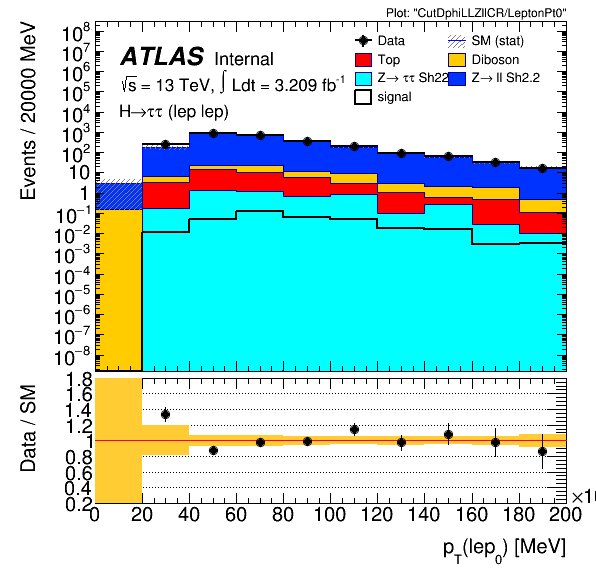
\includegraphics[width=0.4\textwidth]{figures/v05/sherpa22/eemm-CutDphiLLZllCR-LeptonPt0-log}
   }
   \caption{Distibutions in Nominal Z$\rightarrow\ell\ell$ Control region}
  \label{fig:lepPt0ZCR}
\end{figure}



\begin{figure}[h!]
  \centering
   \subfloat[]{  
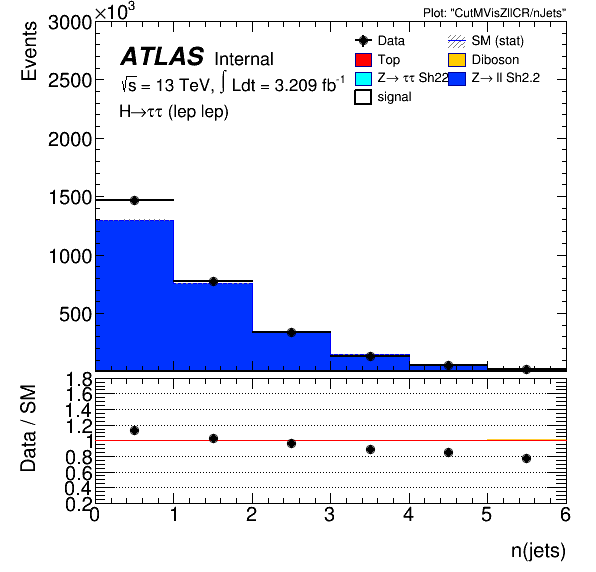
\includegraphics[width=0.4\textwidth]{figures/v05/sherpa22/eemm-CutMVisZllCR-nJets-lin}
   }
   \subfloat[]{  
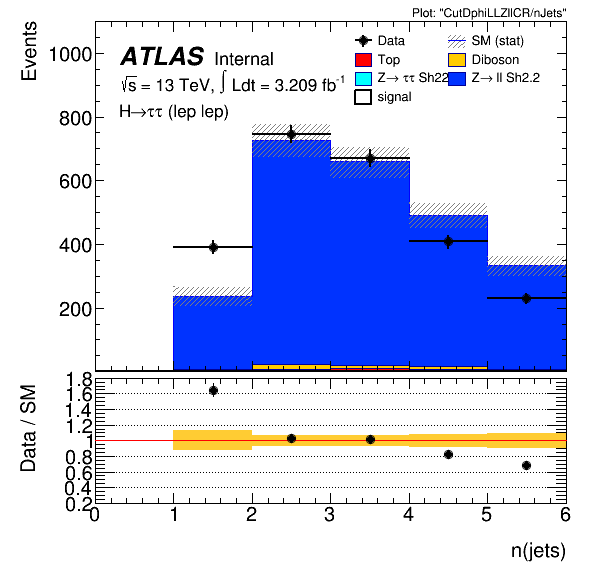
\includegraphics[width=0.4\textwidth]{figures/v05/sherpa22/eemm-CutDphiLLZllCR-nJets-lin}
   }\\
   \subfloat[]{  
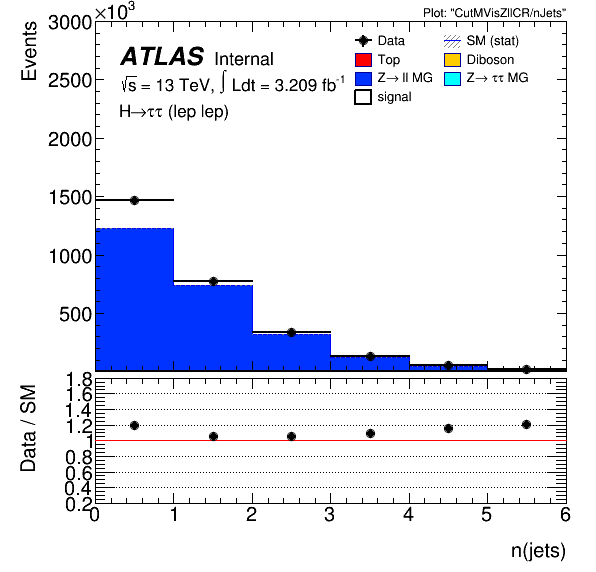
\includegraphics[width=0.4\textwidth]{figures/v05/mg/eemm-CutMVisZllCR-nJets-lin}
   }
   \subfloat[]{  
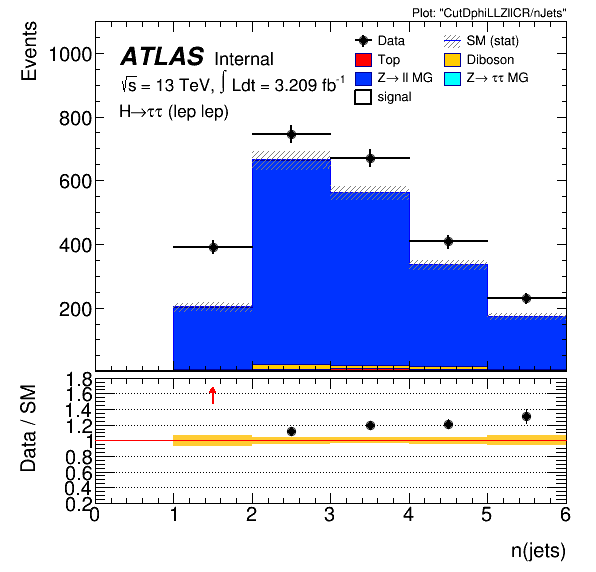
\includegraphics[width=0.4\textwidth]{figures/v05/mg/eemm-CutDphiLLZllCR-nJets-lin}
   }\\
   \subfloat[]{  
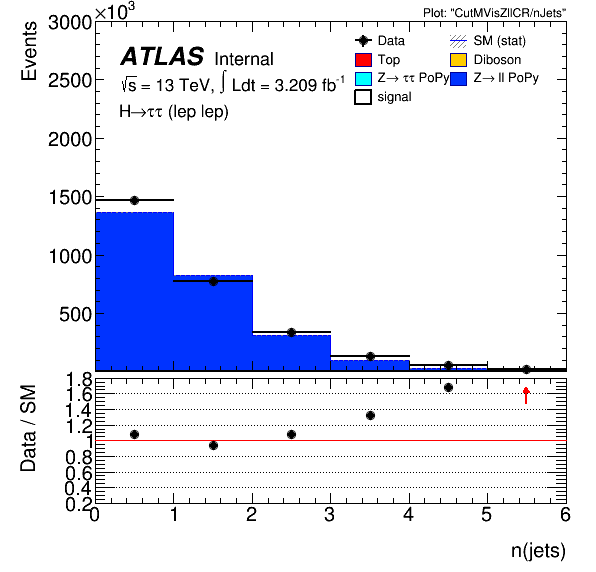
\includegraphics[width=0.4\textwidth]{figures/v05/popy/eemm-CutMVisZllCR-nJets-lin}  
   }
   \subfloat[]{  
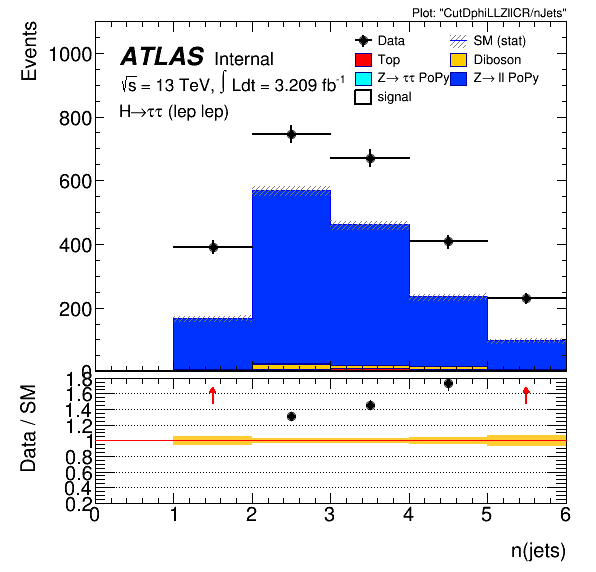
\includegraphics[width=0.4\textwidth]{figures/v05/popy/eemm-CutDphiLLZllCR-nJets-lin}
   }
   \caption{Jet Multiplicity in Base and Contrained Z$\rightarrow\ell\ell$ Control regions}
  \label{fig:lepnJetsZCR}
\end{figure}

\begin{table}[h]
\centering
\begin{tabular}{rrrrrrrr}
\hline
\hline
 &  SR$^{(\mathrm{Preselection})}$ &  M$_{Vis}$ &  E$_\mathrm{T}^{miss}$ &  X$_1$,X$_2$ &  $\Delta\phi_{\ell\ell}$ \\
Sherpa vs PoPy &-58.27 &-58.21 &-43.78 &-38.07 &-28.10\\
Sherpa vs mg &-34.20 &-29.61 &-23.11 &-16.99 &-14.69\\
\hline
TOTAL & $\pm  67.57 $ & $\pm  65.31 $ & $\pm  49.50 $ & $\pm  41.69 $ & $\pm  31.71 $ \\
\hline
\hline
\end{tabular}
\caption{Percentage uncertainties arising from the difference in yields as predicted by different MC generators. The SR column represents the `raw' difference in generators. All others are calculated from the difference in normalisation factors}
\label{table:uncertainties}
\end{table}